% huji_stats_2026.tex — Statistics Department, Hebrew University, June 2026
% "Feature Selection: Benchmark Hardness, Predictive Utility, and Resource Costs"
% Dan Vilenchik, Ben-Gurion University of the Negev
%
% Compile: /Library/TeX/texbin/pdflatex -interaction=nonstopmode -halt-on-error huji_stats_2026.tex
%          (run twice for navigation/labels)
%
% Structure: recap/motivation -> Q1 (predicting FS utility) -> Q2 (resource-aware) .
% Peeling lives in the recap + backup. No speaker notes.

\documentclass[aspectratio=169,10pt,dvipsnames]{beamer}

%% ── Packages ─────────────────────────────────────────────────────────────────
\usepackage{tikz}
\usetikzlibrary{arrows.meta,positioning,shapes.geometric,
                fit,decorations.pathreplacing,backgrounds,calc,patterns}
\usepackage{amsmath,amssymb}
\usepackage{booktabs}
\usepackage{array}
\newcolumntype{R}[1]{>{\raggedright\arraybackslash}p{#1}}
\usepackage{xcolor}
\usepackage{hyperref}

%% ── Theme ────────────────────────────────────────────────────────────────────
\usetheme{Madrid}
\usecolortheme{default}

%% ── BGU colors ───────────────────────────────────────────────────────────────
\definecolor{bgucolor}{RGB}{0,100,130}
\definecolor{bgulight}{RGB}{220,240,245}
\definecolor{bgumid}{RGB}{0,140,180}
\definecolor{emphcolor}{RGB}{180,40,40}
\definecolor{easygreen}{RGB}{38,155,36}
\definecolor{medorange}{RGB}{210,100,0}
\definecolor{hardred}{RGB}{180,0,0}

\setbeamercolor{structure}{fg=bgucolor}
\setbeamercolor{frametitle}{bg=bgucolor,fg=white}
\setbeamercolor{title}{fg=white}
\setbeamercolor{author}{fg=bgucolor}
\setbeamercolor{institute}{fg=black!65}
\setbeamercolor{date}{fg=black!60}
\setbeamercolor{block title}{bg=bgucolor!85,fg=white}
\setbeamercolor{block body}{bg=bgucolor!10}
\setbeamercolor{alerted text}{fg=emphcolor}
\setbeamerfont{frametitle}{series=\bfseries}
\setbeamerfont{block title}{series=\bfseries}

%% ── Clickable links ──────────────────────────────────────────────────────────
\hypersetup{colorlinks=true,urlcolor=bgumid,linkcolor=bgumid,citecolor=bgumid}

\newcommand{\kbsfull}{Itamar Elmakias \& Dan Vilenchik,
  ``Choosing the Right Dataset: Hardness Criteria for Feature Selection
  Benchmarking,'' \emph{Knowledge-Based Systems} \textbf{334}, 115022 (2026).}
\newcommand{\kbsdoi}{\href{https://doi.org/10.1016/j.knosys.2025.115022}%
  {doi.org/10.1016/j.knosys.2025.115022}}
\newcommand{\kbssd}{\href{https://www.sciencedirect.com/science/article/abs/pii/S095070512502060X}%
  {ScienceDirect}}
\newcommand{\repo}{\href{https://github.com/Itamarelmakia/FeatureSelect-Benchmark-Hub}%
  {\texttt{github.com/Itamarelmakia/FeatureSelect-Benchmark-Hub}}}

%% ── Exclude backup slides from the footer count ──────────────────────────────
%% Replicates appendixnumberbeamer without the external package: at \appendix we
%% record the main-body frame count into the .aux (read back on the next run) and
%% drop the footer on backup frames.
\makeatletter
\newcommand{\mainframetotal}{\inserttotalframenumber}
\apptocmd{\appendix}{%
  \immediate\write\@auxout{\string\gdef\string\mainframetotal{\the\value{framenumber}}}%
  \setbeamertemplate{footline}{}%
}{}{}
\makeatother

%% ── Compact footer ───────────────────────────────────────────────────────────
\setbeamertemplate{footline}{%
  \hfill\usebeamercolor[fg]{structure}\small
  \insertframenumber\,/\,\mainframetotal\hspace{6pt}\vspace{4pt}%
}
\setbeamertemplate{navigation symbols}{}

%% ── TikZ styles ──────────────────────────────────────────────────────────────
\tikzset{
  box/.style    = {draw=bgucolor,rounded corners=4pt,fill=bgulight,
                   text width=3.0cm,align=center,font=\small,inner sep=6pt},
  wbox/.style   = {draw=bgucolor,rounded corners=4pt,fill=white,
                   text width=3.0cm,align=center,font=\small,inner sep=6pt},
  arrow/.style  = {->,>=Stealth,thick,color=bgucolor},
  rdarrow/.style= {->,>=Stealth,thick,color=emphcolor},
  hl/.style     = {draw=emphcolor,thick,rounded corners=3pt,fill=emphcolor!12},
  peel/.style   = {draw=medorange,rounded corners=4pt,fill=medorange!10,
                   text width=2.8cm,align=center,font=\small,inner sep=5pt},
}

%% ── Image path ───────────────────────────────────────────────────────────────
\graphicspath{{assests/}}

%% ── Metadata ─────────────────────────────────────────────────────────────────
\title[FS: hardness, utility, resources]{Feature Selection: Benchmark Hardness, Predictive Utility, and Resource Costs}
\subtitle{From dataset taxonomy to preprocessing decisions}

\author{Dan Vilenchik}

\institute{
Department of Electrical and Computer Engineering\\
Ben-Gurion University of the Negev\\[4pt]
{\small Joint work with Itamar Elmakias (PhD thesis)}
}

\date{\textcolor{blue}{
Department of Statistics Seminar, Hebrew University, 
June 2026}}
%% ═══════════════════════════════════════════════════════════════════════════════
\begin{document}
%% ═══════════════════════════════════════════════════════════════════════════════

%% ── TITLE ────────────────────────────────────────────────────────────────────
{
\setbeamertemplate{footline}{}
\begin{frame}
  \vspace{0.5cm}
  \titlepage
  \vspace{-0.4cm}
  \begin{center}
    \small\color{bgucolor!80}
  \end{center}
\end{frame}
}

%% ══════════════════════════════════════════════════════════════════════════════
%%  PART 1 — RECAP & MOTIVATION
%% ══════════════════════════════════════════════════════════════════════════════
\section{Recap and Motivation}

%% ── Recap 1 ──────────────────────────────────────────────────────────────────
\begin{frame}{Recap: dataset hardness for feature-selection benchmarks}
\begin{columns}[T]
\column{0.55\textwidth}
\vspace{0.2cm}
Feature selection (FS) is a standard pipeline step, with dozens of algorithms.
We benchmark them on commonly used datasets --- but
\alert{are those datasets meaningful?}

\medskip
We built a hardness framework: run 37 FS algorithms on 102 datasets
(63 binary, 39 multi-class) and label each dataset by the best AUC achievable.
\begin{itemize}
  \item \textcolor{easygreen}{\textbf{Easy}}: best AUC $\geq 90\%$
  \item \textcolor{medorange}{\textbf{Medium}}: $70$--$90\%$
  \item \textcolor{hardred}{\textbf{Hard}}: $< 70\%$
\end{itemize}

\pause
\column{0.43\textwidth}
\vspace{0.1cm}
\centering
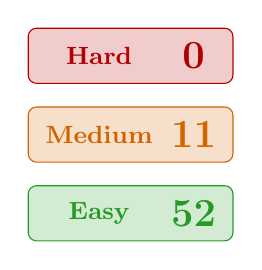
\begin{tikzpicture}
  \foreach \y/\col/\lab/\cnt in {
    2.4/hardred/Hard/0,
    1.4/medorange/Medium/11,
    0.4/easygreen/Easy/52}{
    \fill[\col!20,draw=\col,rounded corners=3pt]
      (0,\y) rectangle (2.6,\y+0.7);
    \node[font=\small\bfseries,color=\col] at (0.9,\y+0.35) {\lab};
    \node[font=\Large\bfseries,color=\col] at (2.1,\y+0.35) {\cnt};
  }
\end{tikzpicture}

\vspace{4pt}
{\small 63 binary datasets.\\
\textbf{No} dataset is Hard under this protocol.}
\end{columns}

\vspace{0.3cm}
{\footnotesize\color{bgucolor!80} Published in \emph{Knowledge-Based Systems}
\textbf{334}, 115022 (2026). \kbsdoi}
\end{frame}

%% ── Recap 2 ──────────────────────────────────────────────────────────────────
\begin{frame}{High-dimensional theory predicts that hard instances should exist}
\begin{columns}[T]
\column{0.49\textwidth}
\vspace{0.2cm}
\textbf{Spiked covariance model} (Johnstone; Baik--Ben Arous--P\'ech\'e):
\[
  X_i = \sqrt{\lambda}\,z_i\,\mathbf{v} + \boldsymbol{\varepsilon}_i,\quad
  \mathbf{v}\in\mathbb{R}^p,\; z_i\sim\mathcal{N}(0,1)
\]
Recovering the signal $\mathbf{v}$ has a sharp phase transition at
$\lambda_c = \sqrt{p/n}$:
\begin{itemize}
  \item $\lambda < \lambda_c$: the leading sample eigenvector is asymptotically
        orthogonal to $\mathbf{v}$ --- PCA carries no signal
  \item $\lambda > \lambda_c$: alignment emerges
\end{itemize}

\medskip
{\small Related high-dimensional recovery problems exhibit provable hard regimes
(sparse PCA: Berthet--Rigollet; Krauthgamer--Nadler--V., \emph{Ann.\ Stat.} 2015),
which motivates expecting hard FS-like regimes.}

\pause
\column{0.49\textwidth}
\centering
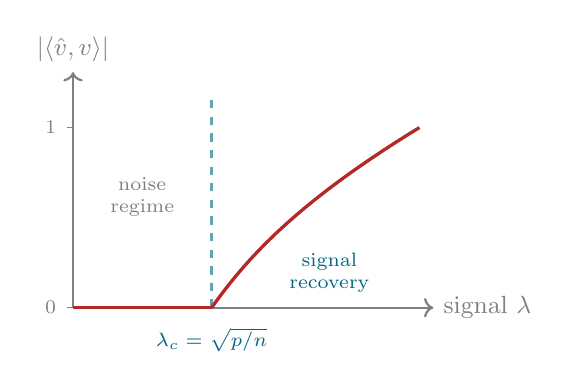
\begin{tikzpicture}[scale=0.88]
  \draw[->,thick,gray] (0,0) -- (5.2,0) node[right,font=\small] {signal $\lambda$};
  \draw[->,thick,gray] (0,0) -- (0,3.4)
        node[above,font=\small] {$|\langle\hat{v},v\rangle|$};
  \draw[dashed,bgucolor!60,thick] (2,0) -- (2,3.0);
  \node[below,font=\scriptsize,bgucolor] at (2,-0.15) {$\lambda_c=\sqrt{p/n}$};
  \draw[emphcolor,very thick] (0,0) -- (2,0);
  \draw[emphcolor,very thick]
        (2,0) .. controls (2.5,0.7) and (3.2,1.5) .. (5,2.6);
  \node[font=\scriptsize,gray,align=center] at (1.0,1.6) {noise\\regime};
  \node[font=\scriptsize,bgucolor,align=center] at (3.7,0.5) {signal\\recovery};
  \foreach \y/\lab in {0/0,2.6/1}{
    \draw[gray,thin] (-0.08,\y) -- (0,\y);
    \node[left,font=\scriptsize,gray] at (-0.1,\y) {\lab};
  }
\end{tikzpicture}

\vspace{4pt}
{\small\textit{Below $\lambda_c$, the leading eigenvector is uninformative.}}
\end{columns}
\end{frame}

%% ── Recap 3 ──────────────────────────────────────────────────────────────────
\begin{frame}{Empirical benchmarks often do not exhibit the predicted difficulty}
\begin{columns}[T]
\column{0.48\textwidth}
\vspace{0.2cm}
Theory predicts: when $p/n$ is large, FS should be unreliable.
Many of our 102 datasets are high-dimensional ($p \gg n$).

\pause
\medskip
What we observe:
\begin{itemize}
  \item No significant correlation between $p/n$ and performance
  \item No significant correlation between class imbalance and performance
  \item Many ``high-dimensional'' datasets are \textcolor{easygreen}{\textbf{Easy}}
\end{itemize}

\medskip
{\small The hard regime exists in theory but is largely absent from the datasets
commonly used for FS benchmarking.}

\column{0.48\textwidth}
\centering
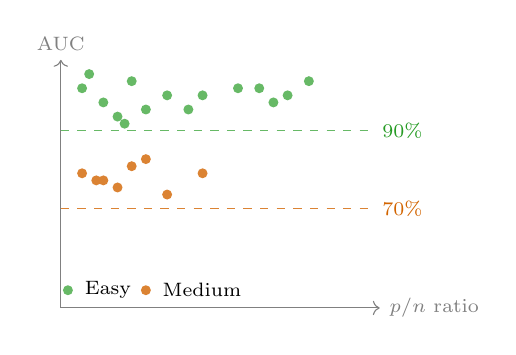
\begin{tikzpicture}[scale=0.9]
  \draw[->,thin,gray] (0,0) -- (4.5,0) node[right,font=\scriptsize] {$p/n$ ratio};
  \draw[->,thin,gray] (0,0) -- (0,3.5) node[above,font=\scriptsize] {AUC};
  \foreach \x/\y in {0.3/3.1, 0.6/2.9, 1.0/3.2, 1.5/3.0, 0.8/2.7,
                      1.8/2.8, 2.5/3.1, 3.0/2.9, 3.5/3.2, 0.4/3.3,
                      2.0/3.0, 1.2/2.8, 2.8/3.1, 0.9/2.6, 3.2/3.0}{
    \fill[easygreen!70] (\x,\y) circle (2pt);
  }
  \foreach \x/\y in {0.5/1.8, 1.0/2.0, 1.5/1.6, 2.0/1.9, 0.8/1.7,
                      1.2/2.1, 0.3/1.9, 0.6/1.8}{
    \fill[medorange!80] (\x,\y) circle (2pt);
  }
  \draw[dashed,easygreen!70,thin] (0,2.5) -- (4.4,2.5)
        node[right,font=\scriptsize,easygreen] {90\%};
  \draw[dashed,medorange!80,thin] (0,1.4) -- (4.4,1.4)
        node[right,font=\scriptsize,medorange] {70\%};
  \fill[easygreen!70] (0.1,0.25) circle (2pt);
  \node[right,font=\scriptsize] at (0.2,0.25) {Easy};
  \fill[medorange!80] (1.2,0.25) circle (2pt);
  \node[right,font=\scriptsize] at (1.3,0.25) {Medium};
\end{tikzpicture}

\vspace{4pt}
{\small\textit{No clear trend: high-$p/n$ datasets are often Easy.}}
\end{columns}
\end{frame}

%% ── Recap 4: peeling motivation/result ───────────────────────────────────────
\begin{frame}{Generating hard benchmark variants by peeling}
\begin{columns}[T]
\column{0.52\textwidth}
\vspace{0.2cm}
Since no naturally occurring Hard binary dataset was identified under the protocol,
the published paper introduces \textbf{peeling}:  \textcolor{easygreen} {shrink a dataset's training set
while keeping a known ground-truth feature set $F$ that still works.}

\medskip
\begin{itemize}
  \item Hard under our protocol: the 37 FS algorithms fail to recover $F$
  \item The retained set $F$ still achieves good AUC, so the variant is not
        merely degraded noise
  \item Certified by construction, not a formal hardness theorem
\end{itemize}

\pause
\medskip
\textbf{Outcome:} peeling all 63 binary datasets produced two Hard datasets ---
Slashdot and SMK-CAN-187.

\column{0.45\textwidth}
\vspace{0.2cm}
\centering
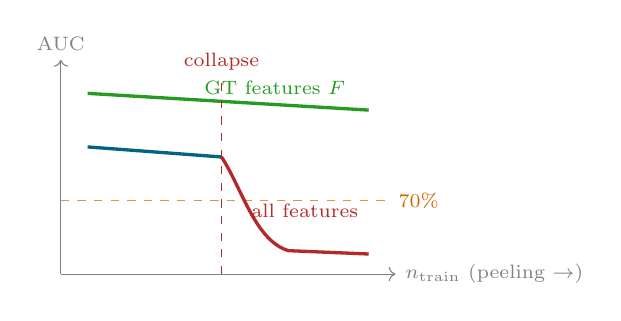
\begin{tikzpicture}[scale=0.85]
  \draw[->,thin,gray] (0,0) -- (5.0,0)
        node[right,font=\scriptsize] {$n_{\text{train}}$ (peeling $\to$)};
  \draw[->,thin,gray] (0,0) -- (0,3.2) node[above,font=\scriptsize] {AUC};
  \draw[dashed,medorange!70,thin] (0,1.1) -- (4.9,1.1)
        node[right,font=\scriptsize,medorange] {70\%};
  \draw[easygreen,very thick] (0.4,2.7) -- (4.6,2.45);
  \node[easygreen,font=\scriptsize,right] at (2.0,2.78) {GT features $F$};
  \draw[bgucolor,very thick] (0.4,1.9) -- (2.4,1.75);
  \draw[emphcolor,very thick]
        (2.4,1.75) .. controls (2.7,1.3) and (2.9,0.5) .. (3.4,0.35) -- (4.6,0.3);
  \node[emphcolor,font=\scriptsize,right] at (2.7,0.95) {all features};
  \draw[emphcolor,dashed,thin] (2.4,0) -- (2.4,2.9)
        node[above,font=\scriptsize,emphcolor] {collapse};
\end{tikzpicture}

\vspace{2pt}
{\small\textit{A possible phase transition in FS recovery.\\
Procedure on the next slide.}}
\end{columns}
\end{frame}

%% ── Recap 5: peeling procedure ───────────────────────────────────────────────
\begin{frame}{The peeling procedure}
\begin{center}
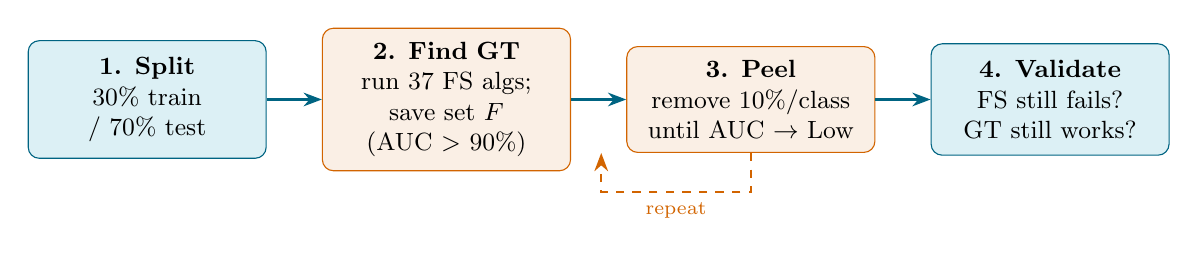
\begin{tikzpicture}[node distance=0.4cm and 0.7cm,every node/.style={font=\small}]
  \node[box,text width=2.6cm] (split) {\textbf{1. Split}\\30\% train / 70\% test};
  \node[peel,right=0.7cm of split] (gt) {\textbf{2. Find GT}\\run 37 FS algs;\\save set $F$ (AUC $>$ 90\%)};
  \node[peel,right=0.7cm of gt] (peel) {\textbf{3. Peel}\\remove 10\%/class\\until AUC $\to$ Low};
  \node[box,text width=2.6cm,right=0.7cm of peel] (val) {\textbf{4. Validate}\\FS still fails?\\GT still works?};
  \draw[arrow] (split) -- (gt);
  \draw[arrow] (gt) -- (peel);
  \draw[arrow] (peel) -- (val);
  \draw[arrow,dashed,medorange] (peel.south) -- ++(0,-0.5) -- ++(-1.9,0)
       node[below,font=\scriptsize,medorange,midway]{repeat} -- ++(0,0.5);
\end{tikzpicture}
\end{center}

\pause
\medskip
\begin{columns}[T]
\column{0.5\textwidth}
\small
\textbf{Stop when} no-FS AUC drops to Low ($<70\%$).\\
\textbf{Fail if} $n<50$ or GT loses discriminative power.

\column{0.47\textwidth}
\small
\textbf{Output:} a dataset that is Hard under our protocol, with a known $F$ that
still recovers good AUC.
\end{columns}

\pause

\medskip

\begin{block}{Open Research Question}

Can we define a generative model that mirrors this process, with interpretable

parameters that explain the success and failure modes of the peeling?

\end{block}


\end{frame}

%% ── Recap 6: the two questions ───────────────────────────────────────────────
\begin{frame}{From benchmark hardness to two follow-up questions}
\begin{center}
So far, we've asked what kind of benchmarks are used in the FS community. We now consider two
follow-up questions.
\end{center}

\vspace{0.3cm}
\begin{columns}[T]
\column{0.48\textwidth}
\begin{block}{Question 1}
\centering
Can we predict whether FS will improve predictive performance?
\end{block}

\pause
\column{0.48\textwidth}
\begin{block}{Question 2}
\centering
Conditional on using FS, which resource dimensions improve performance?
\end{block}
\end{columns}

\pause
\vspace{0.5cm}
\begin{center}
\small\color{bgucolor!80}
\textit{Dataset hardness provides the organizing variable for both questions.}
\end{center}
\end{frame}


%% ══════════════════════════════════════════════════════════════════════════════
%%  CHAPTER 1 — PREDICTING FS UTILITY  (anomaly detection)
%% ══════════════════════════════════════════════════════════════════════════════
\section{Q1: Predicting Feature-Selection Utility}

{
\setbeamercolor{background canvas}{bg=bgucolor!8}
\begin{frame}
\vspace{1.6cm}
\begin{center}
{\Large\bfseries\color{bgucolor} Question 1}\\[8pt]
{\large Predicting feature-selection utility}\\[16pt]
\small\color{gray}
\textit{Can dataset descriptors identify when FS improves predictive performance?}
\end{center}
\end{frame}
}

%% ── C1.1a: prior work / what has been done ────────────────────────────────────
\begin{frame}{Prior work established that FS benefit is dataset-dependent}
\vspace{0.2cm}
\begin{itemize}
  \item \textbf{Surveys / benchmarks} show no universally best FS method;
        outcomes depend on the dataset and the learner
        (Bommert et al.\ 2020; Li et al.\ 2017).
  \item \textbf{Meta-learning} predicts FS choices from dataset
        descriptors (Filchenkov \& Pendryak 2015; Parmezan et al.\ 2017).
  \item \textbf{Post et al.\ (2016)} predicts
        whether  Correlation-based Feature Subset Selection (CfsSubsetEval) improves AUC for a \emph{dataset~$\times$~classifier} pair,
        across 394 OpenML binary datasets and 12 classifiers, using a
        Random-Forest meta-model.
\end{itemize}


\end{frame}

%% ── C1.1b: closest work and how we differ ─────────────────────────────────────
\begin{frame}{Relation to Post et al.\ (2016)}


\centering
\footnotesize
\renewcommand{\arraystretch}{1.35}
\setlength{\tabcolsep}{8pt}
\begin{tabular}{@{}p{2.3cm}p{4.8cm}p{4.8cm}@{}}
\toprule
 & \textbf{Post et al.\ (2016)} & \textbf{This work} \\
\midrule
Question
& Does FS improve a specified classifier on this dataset?
& Is FS worthwhile for this dataset? \\

Decision unit
& Dataset $\times$ classifier
& Dataset-level screening decision \\

FS intervention
& One CFS subset-selection method
& 37 FS algorithms across multiple subset sizes \\

Utility label
& Any / statistically significant improvement
& Meaningful gain ($\Delta$AUC $\geq 0.05$) \\

Learning paradigm
& Supervised meta-learning over labeled dataset--classifier pairs
& Rare-event detection + weak-positive supervised transfer \\

Positive class
& 41\% of pairs improve; 10\% significantly
& 7/102 datasets exhibit substantial oracle gain \\

Best AUROC
& 0.77--0.78
& above 0.90  \\

\bottomrule
\end{tabular}

\end{frame}

%% ── C1.2 ─────────────────────────────────────────────────────────────────────
\begin{frame}{Oracle estimate of feature-selection utility}
\begin{columns}[T]
\column{0.54\textwidth}
\vspace{0.2cm}
\textbf{Setup:} 37 FS algorithms $\times$ 102 datasets $\times$ 5 classifiers.\\

\medskip
For each dataset $\mathcal{D}_i$,
\[
  \Delta\mathrm{AUC}(\mathcal{D}_i) = \mathrm{AUC}^{\text{FS}} - \mathrm{AUC}^{\text{no-FS}},
\]
where $\mathrm{AUC}^{\text{FS}}$ is the best result over all algorithms,
classifiers, and feature counts $K$.

\medskip
\textbf{Threshold:} $\Delta\mathrm{AUC} \geq 0.05$ counts as a substantial gain.

\pause
\column{0.43\textwidth}
\vspace{0.2cm}
The oracle is deliberately conservative (w.r.t FP rate) as it selects, in hindsight, the best
\begin{itemize}
  \item algorithm,
  \item number of features $K$,
  \item classifier
\end{itemize}
per dataset.

\medskip
{\small If gains are uncommon under this oracle evaluation, they are unlikely to
be common under ordinary model-selection constraints.}
\end{columns}
\end{frame}

%% ── C1.3 ─────────────────────────────────────────────────────────────────────
\begin{frame}{Substantial predictive gains are rare in this benchmark}
\begin{columns}[T]
\column{0.56\textwidth}
\centering
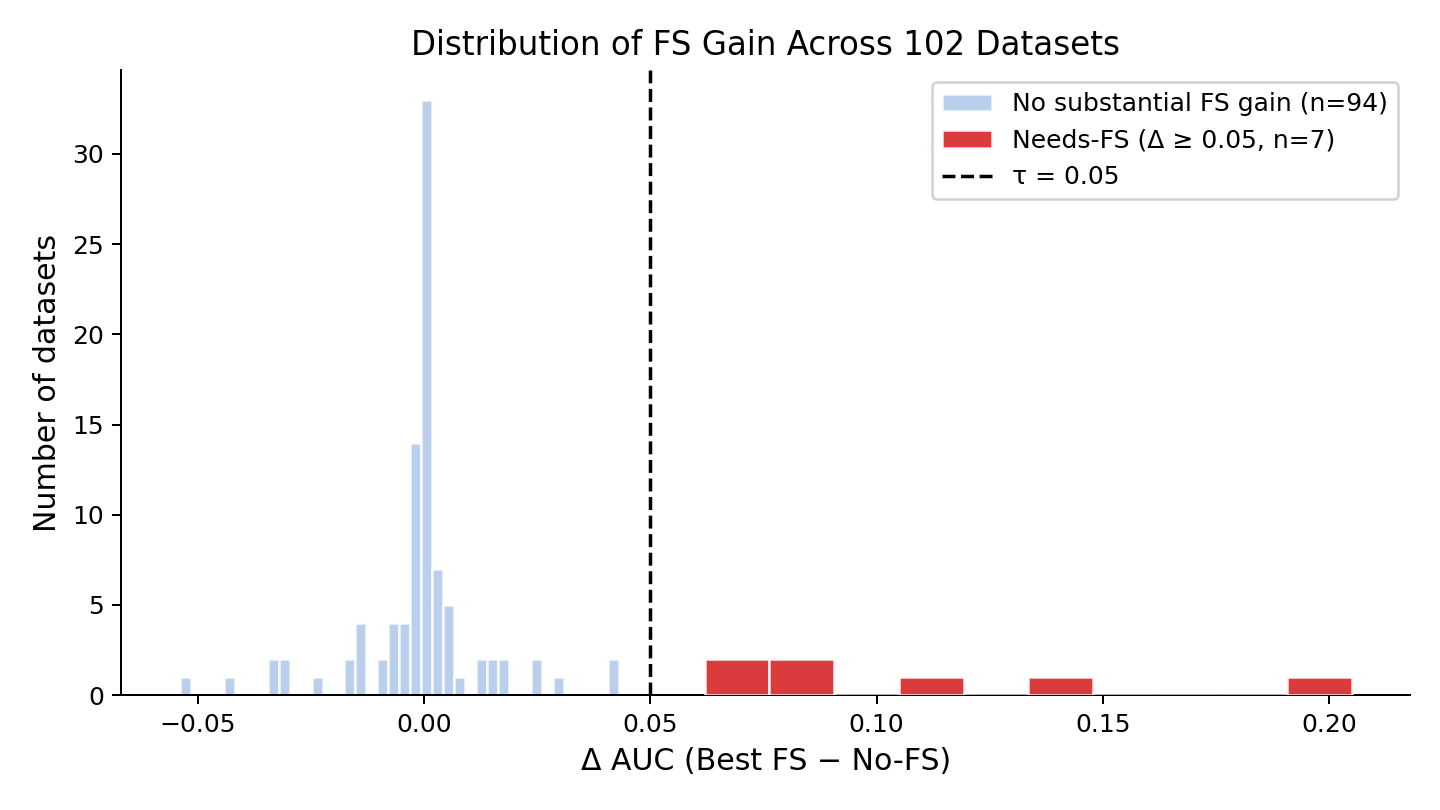
\includegraphics[width=\linewidth]{Paper3_Itamar/assets/delta_auc_histogram.png}



\pause
\column{0.42\textwidth}
\vspace{0.3cm}
Only \textbf{7 of 102} datasets (6.9\%) reach $\Delta\mathrm{AUC}\geq 0.05$ ---
even under the generous oracle.

\medskip
\begin{itemize}
  \item Most datasets cluster near $\Delta = 0$
  \item Some show lower AUC after FS
  \item Those datasets account for under 1\% of the total FS search
cost
\end{itemize}


\end{columns}
\end{frame}

\begin{frame}{Dataset Representation: Intrinsic Complexity Descriptors}

\small
\begin{table}
\centering
\renewcommand{\arraystretch}{1.2}
\begin{tabular}{p{3.5cm}p{6.8cm}}
\toprule
\textbf{Feature group} & \textbf{Examples} \\
\midrule
Basic meta-features &
\#Samples, \#Features, Feature/Sample ratio, Class imbalance \\

Baseline performance &
Probe\_AUC$_0$ (classifier without feature selection) \\

\textbf{Problexity descriptors} &
\textbf{F1}: Fisher's discriminant ratio (single-feature separability)\\
&
\textbf{F1v}: Directional Fisher criterion (multivariate linear separability)\\
&
\textbf{N2}: Ratio of intra-/inter-class nearest-neighbor distances\\
&
\textbf{N3}: 1-NN leave-one-out error (local neighborhood complexity)\\
&
Class overlap and decision-boundary geometry \\
\bottomrule
\end{tabular}
\end{table}


\pause

\medskip
\alert{Unlike prior work, our representation relies on intrinsic dataset geometry rather than
classifier or feature-selection landmarkers.}

\end{frame}

%% ── C1.4 ─────────────────────────────────────────────────────────────────────
\begin{frame}{Beneficial datasets differ in geometry, not raw dimensionality}
\begin{columns}[T]
\column{0.56\textwidth}
\centering
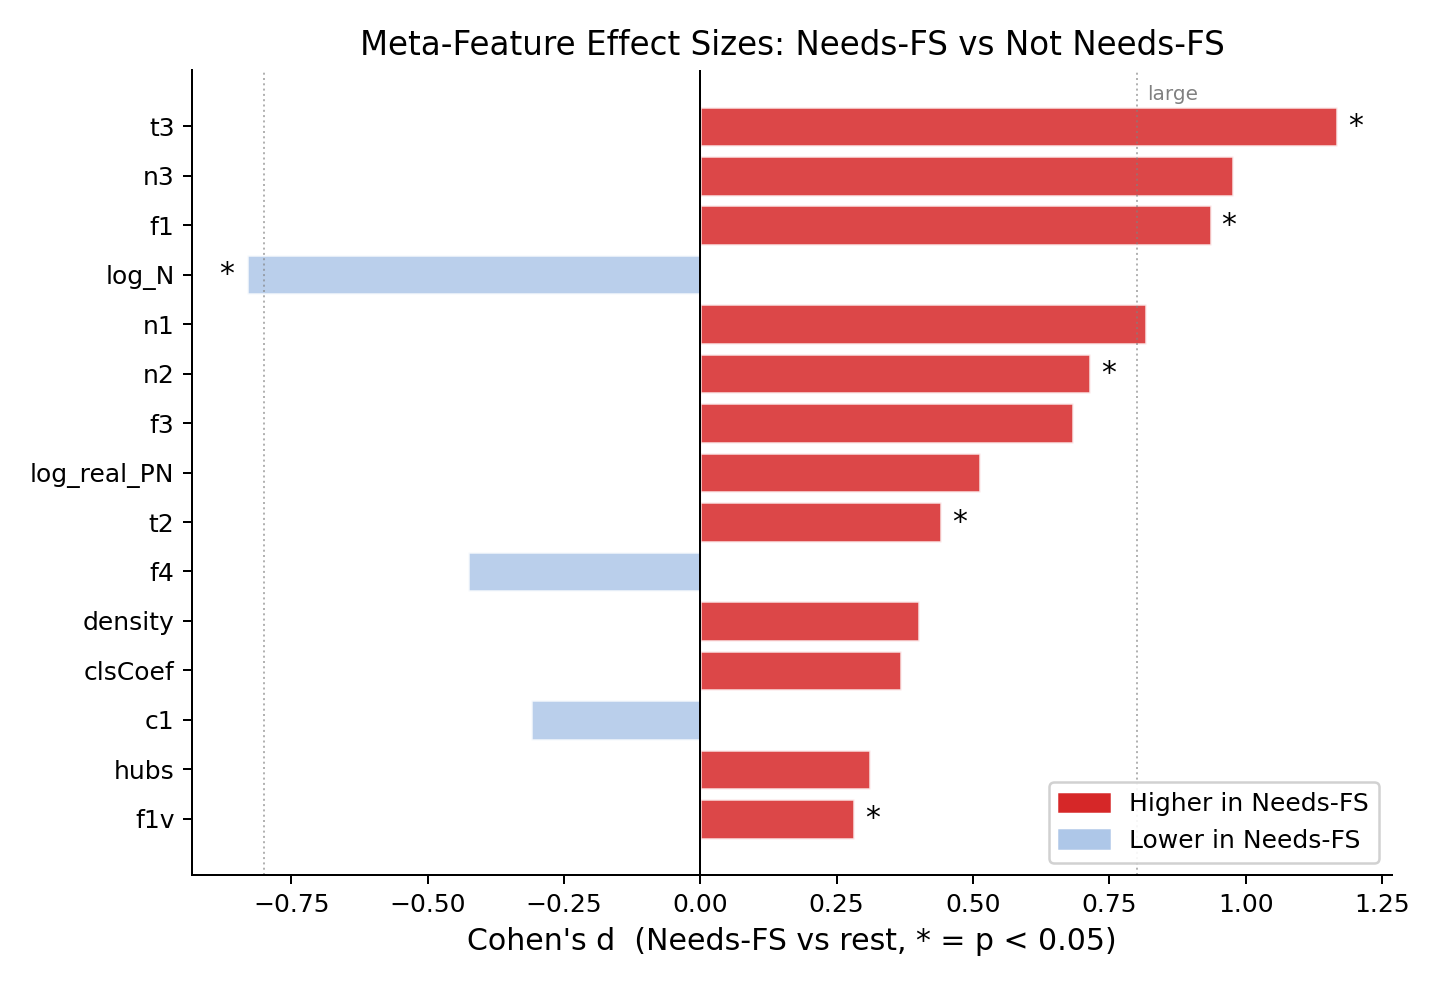
\includegraphics[width=\linewidth]{Paper3_Itamar/assets/top_feature_effect_sizes.png}

\column{0.42\textwidth}
\vspace{0.3cm}
Effect sizes (Cohen's $d$), Needs-FS vs.\ the rest:
\begin{itemize}
  \item Lower baseline AUC (more headroom)
  \item More class overlap
  \item More complex boundary geometry
  \item Smaller sample size
\end{itemize}

\medskip
{\small These descriptors are consistent with the difficulty descriptors used in
the hardness taxonomy.}

\end{columns}
\end{frame}

%% ── C1.6 ─────────────────────────────────────────────────────────────────────
\begin{frame}{One-class detection of beneficial datasets}
\begin{columns}[T]
\column{0.5\textwidth}
\vspace{0.2cm}
\textbf{One-class setup:}
\begin{itemize}
  \item Train on only the 95 No-FS datasets
  \item Test on 7 Needs-FS + 7 random No-FS
  \item Repeat 50 times
\end{itemize}

\medskip
Models: PCA reconstruction, autoencoder, One-Class SVM, LOF (Local Outlier Factor), Isolation Forest.

\medskip
{\small\color{gray} No positive examples are used in training; the detector models
the majority population and flags deviations.}

\pause
\column{0.48\textwidth}
\centering
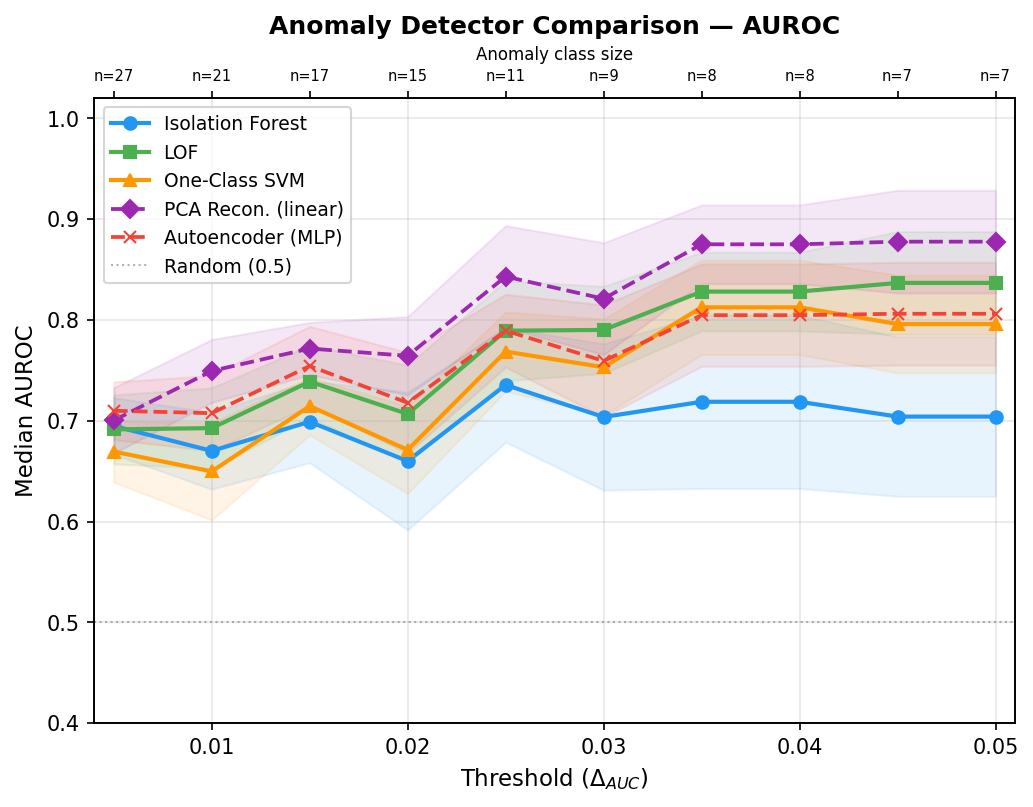
\includegraphics[width=\linewidth]{Paper3_Itamar/assets/ad_auroc_curves.png}
\end{columns}
\end{frame}

%% ── C1.7 ─────────────────────────────────────────────────────────────────────

\begin{frame}{One-class detection of feature-selection-beneficial datasets}

\centering
\footnotesize
\renewcommand{\arraystretch}{1.2}

\begin{tabular}{lcc}
\toprule
\textbf{Model} & \textbf{AUROC} & \textbf{Recall} \\
\midrule
Autoencoder        & 0.90 & 0.71 \\
PCA Reconstruction & 0.89 & 0.86 \\
OC-SVM             & 0.89 & 0.86 \\
LOF                & 0.87 & 0.71 \\
Isolation Forest   & 0.80 & 0.29 \\
\midrule
Random baseline    & 0.50 & -- \\
\bottomrule
\end{tabular}




\end{frame}


\begin{frame}{Weak positive examples improve supervised utility prediction}
\begin{columns}[T]
\column{0.52\textwidth}
\centering
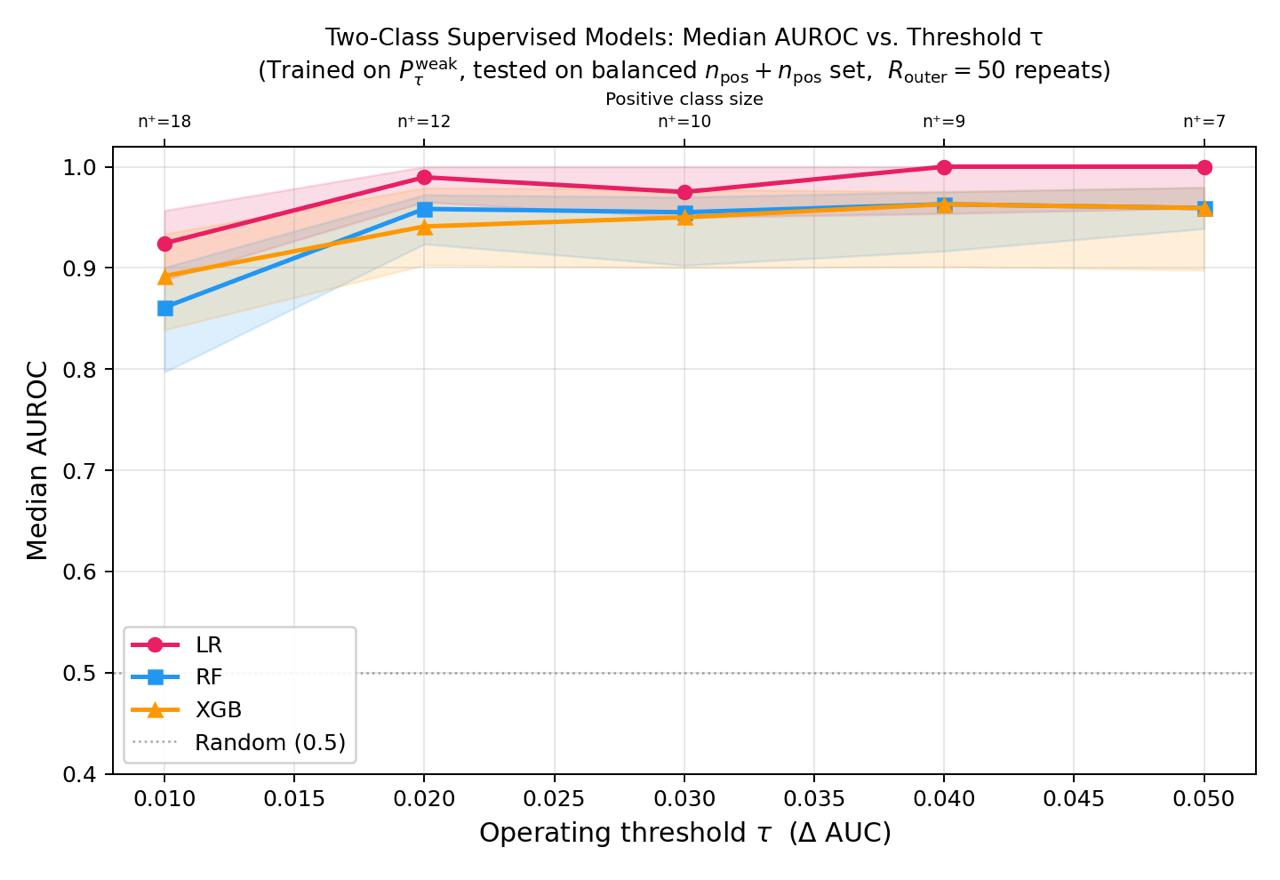
\includegraphics[width=\linewidth]{Paper3_Itamar/assets/twoclass_auroc_vs_tau.jpeg}

\column{0.45\textwidth}
\vspace{1.2cm}
Use weakly beneficial datasets as positives:
\begin{itemize}
  \item Train positives: $0.01 \leq \Delta\mathrm{AUC} < 0.05$
  \item Test positives: $\Delta\mathrm{AUC} \geq 0.05$ (held out)
\end{itemize}

\pause
\medskip
In this evaluation, logistic regression achieves AUROC $1.00$; RF and XGBoost
reach $0.96$; no positive test cases are missed.


\end{columns}
\end{frame}

%% ── C1.9 ─────────────────────────────────────────────────────────────────────
\begin{frame}{Intrinsic descriptors outperform provenance labels}
\begin{columns}[T]
\column{0.48\textwidth}
\vspace{0.2cm}
Does the model rely on dataset provenance (e.g.\ genomic data)?
\begin{center}
\small
\begin{tabular}{lc}
\toprule
Feature representation & AUROC \\
\midrule
Intrinsic descriptors & 1.00 \\
Domain / provenance only & 0.28 \\
Combined & 1.00 \\
\bottomrule
\end{tabular}
\end{center}



\pause
\column{0.50\textwidth}
\centering
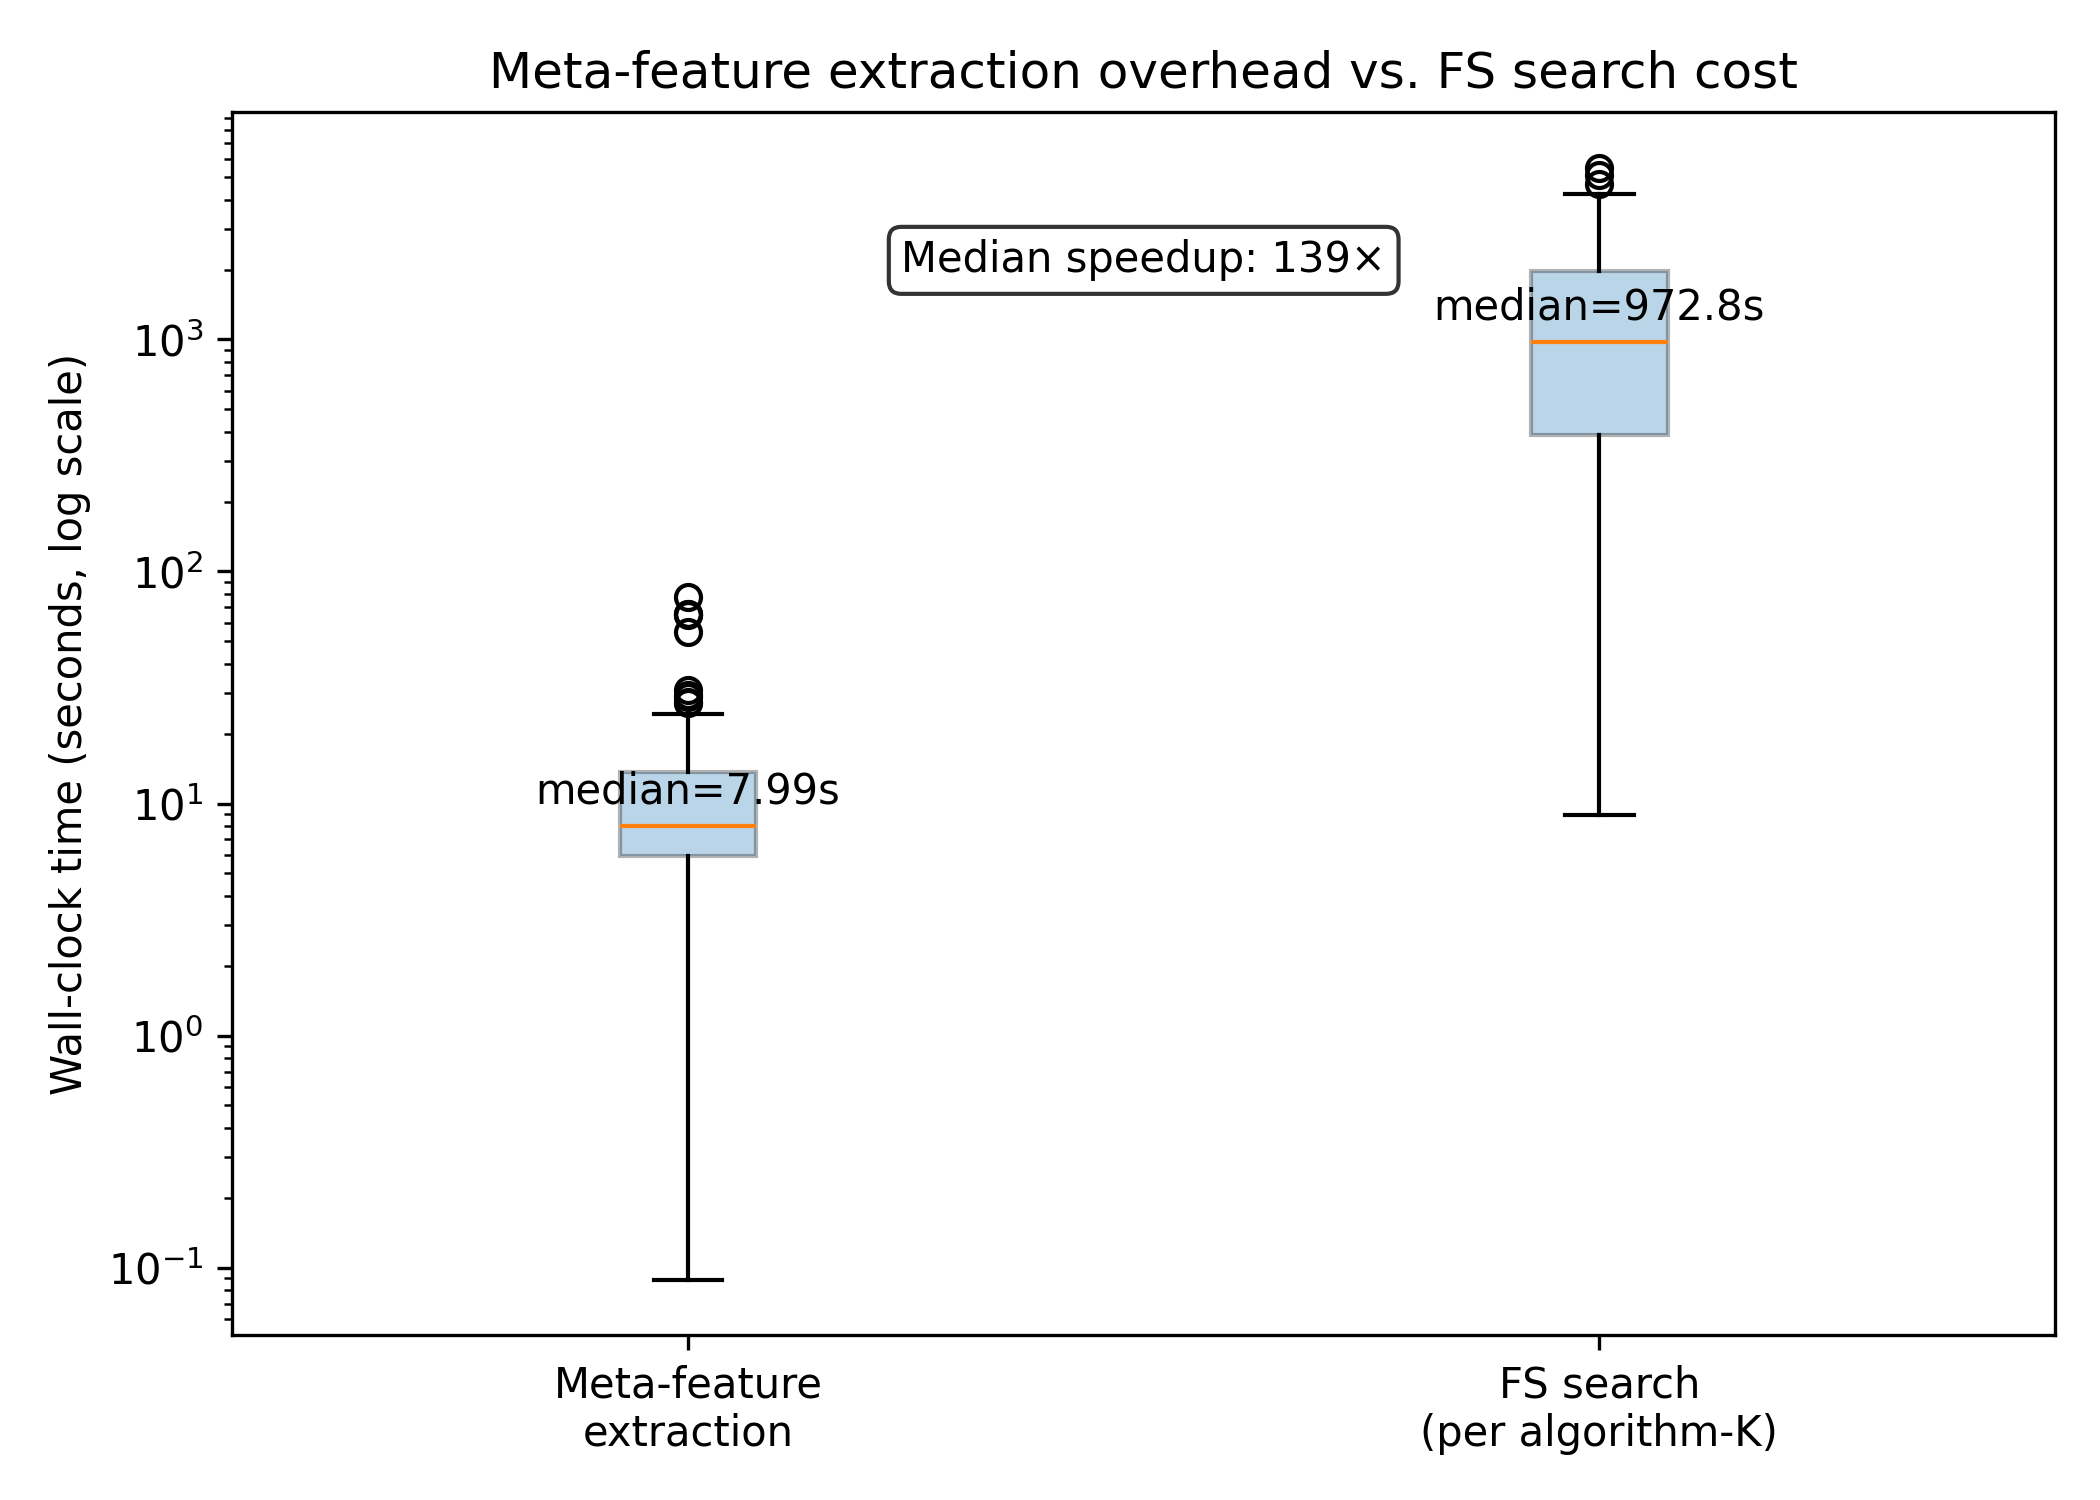
\includegraphics[width=0.95\linewidth]{Paper3_Itamar/assets/gatekeeper_vs_fs_boxplot.png}

\vspace{2pt}
{\small Meta-feature screening has substantially lower median runtime than a
single FS evaluation ($\approx 8$\,s vs.\ $\approx 973$\,s; median ratio
$\approx 139$).}
\end{columns}
\end{frame}


%% ══════════════════════════════════════════════════════════════════════════════
%%  CHAPTER 2 — RESOURCE-AWARE EVALUATION
%% ══════════════════════════════════════════════════════════════════════════════
\section{Q2: Resource-Aware Evaluation}

{
\setbeamercolor{background canvas}{bg=bgucolor!8}
\begin{frame}
\vspace{1.6cm}
\begin{center}
{\Large\bfseries\color{bgucolor} Question 2}\\[8pt]
{\large Resource-aware evaluation of feature-selection methods}\\[16pt]
\small\color{gray}
\textit{Which resource dimensions are associated with improved performance?}
\end{center}
\end{frame}
}

%% ── C2.0: prior work / positioning ────────────────────────────────────────────
\begin{frame}{Prior work gives per-dataset winners, not transparent rules}

\vspace{0.41cm}

\begin{itemize}
  \item \textbf{Surveys / benchmarks} compare algorithms across datasets and
        report \emph{dataset-specific winners} --- no single method dominates
        (Bommert et al.\ 2019/2020).
  \item \textbf{Meta-learning} predicts the best FS method \emph{per dataset}
        from meta-features (Filchenkov 2015; Parmezan et al.\ 2017): a separate
        single-point prediction for each dataset.
  \item \textbf{Complexity descriptors} (e.g.\ Problexity) are high-dimensional
        and highly dataset-specific.
\end{itemize}

\pause
\vspace{0.15cm}
\begin{block}{Practical challenge}
Practitioners need simple rules of thumb:
\emph{When is a lightweight FS method sufficient, and when is additional
investment in runtime, supervision, or custom implementations actually worthwhile?}
\end{block}


\end{frame}

%% ── C2.1 ─────────────────────────────────────────────────────────────────────
\begin{frame}{Grouping methods by resource cost}
\begin{columns}[T]
\column{0.5\textwidth}
\vspace{0.2cm}
37 algorithms, 102 datasets, 5 classifiers.

\medskip
Rather than ranking individual algorithms only, we group methods by resource cost
and test whether higher-cost categories yield systematic gains.

\medskip
Paired within-dataset comparisons:
Wilcoxon signed-rank tests, win rates, Cliff's $\delta$.

\pause
\column{0.47\textwidth}
\vspace{0.2cm}
\textbf{Five resource dimensions:}
\begin{enumerate}
  \item Runtime (fast / moderate / slow)
  \item Implementation (library / research code)
  \item Supervision (supervised / unsupervised)
  \item Method family (filter / wrapper / embedded / \ldots)
  \item Optimization effort (All vs.\ Best)
\end{enumerate}
\end{columns}
\end{frame}

%% ── C2.2: All vs Best (clarify before plots) ─────────────────────────────────
\begin{frame}{Two ways to use FS: ``All'' vs.\ ``Best''}
\begin{columns}[T]
\column{0.48\textwidth}
\centering
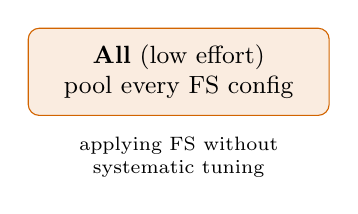
\begin{tikzpicture}[scale=0.9]
  \node[box,fill=medorange!12,draw=medorange,text width=3.4cm] (all)
    {\textbf{All} (low effort)\\\small pool every FS config};
  \node[font=\scriptsize,below=0.15cm of all,text width=3.6cm,align=center]
    {applying FS without systematic tuning};
\end{tikzpicture}

\pause
\column{0.48\textwidth}
\centering
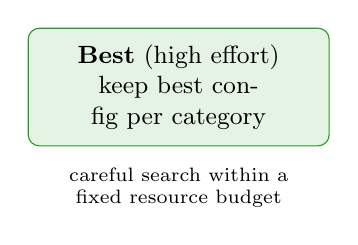
\begin{tikzpicture}[scale=0.9]
  \node[box,fill=easygreen!12,draw=easygreen,text width=3.4cm] (best)
    {\textbf{Best} (high effort)\\\small keep best config per category};
  \node[font=\scriptsize,below=0.15cm of best,text width=3.6cm,align=center]
    {careful search within a fixed resource budget};
\end{tikzpicture}
\end{columns}

\pause
\vspace{0.4cm}
We also split results by hardness (Paper~1 taxonomy). Using the 37-algorithm suite,
the binary split is \textbf{48 Easy / 15 Medium}


\vspace{0.25cm}
\begin{center}
\small\color{bgucolor!80}\textit{The distinction is important because aggregate
conclusions differ across these two regimes.}
\end{center}

\vspace{0.2cm}
\begin{center}
\small\color{black!70}
Medium `Best'-setting results should be interpreted cautiously: only 15 paired datasets, so a
non-significant Medium comparison means ``no evidence of a difference,'' not
``no difference.''
\end{center}
\end{frame}

%% ── C2.3 ─────────────────────────────────────────────────────────────────────
\begin{frame}{Untuned FS configurations underperform the no-FS baseline}
\begin{center}
\includegraphics[width=0.64\linewidth]%
{Feature_Selection_Article2_Itamar/assets/figures/latex_final_boxplots/runtime_bucket__Fig_1__Core__All__Performance_large.png}
\end{center}


\end{frame}

%% ── C2.4 ─────────────────────────────────────────────────────────────────────
\begin{frame}{Longer runtime does not yield systematic AUC gains}
\begin{columns}[T]
\column{0.56\textwidth}
\centering
\includegraphics[width=0.96\linewidth]%
  {Feature_Selection_Article2_Itamar/assets/figures/latex_final_boxplots/runtime_bucket__Fig_2__Core__Best__Performance_large.png}

{\footnotesize Core datasets, ``Best'' setting, by runtime bucket.}

\pause
\column{0.42\textwidth}
\vspace{0.4cm}
Slow methods do not outperform fast ones.
\begin{itemize}
  \item Cliff's $\delta = 0.72$ on Easy (paired comparisons favor fast methods)
  \item Same direction on Medium, but with $n=15$ the test is underpowered;
        we report it as a consistent trend, not a significant effect
\end{itemize}

\medskip
{\small On Easy datasets we find no evidence that higher runtime improves
predictive performance; the direction holds across All and Best.}
\end{columns}
\end{frame}

%% ── C2.5 ─────────────────────────────────────────────────────────────────────
\begin{frame}{Library implementations are more robust in this benchmark}
\begin{center}
\includegraphics[width=0.61\linewidth]%
  {Feature_Selection_Article2_Itamar/assets/figures/latex_final_boxplots/adoption__Fig_1__Performance__All_large.png}
\end{center}

\vspace{-2pt}
\pause
\begin{columns}[T]
\column{0.54\textwidth}
\small
\textbf{Easy (All):} library 93.5\% vs.\ research code 83.1\%.\\
\textbf{Medium (All):} 60.4\% vs.\ 56.6\%.\\
The gap is larger on Medium datasets.

\column{0.42\textwidth}
\small
Research-code implementations are more sensitive to suboptimal settings; a
plausible explanation is that maintained implementations have more stable defaults
and broader testing.
\end{columns}
\end{frame}

%% ── C2.6 ─────────────────────────────────────────────────────────────────────
\begin{frame}{Supervision is the main positive resource effect}
\begin{center}
\includegraphics[width=0.55\linewidth]%
  {Feature_Selection_Article2_Itamar/assets/figures/latex_final_boxplots/supervision__Fig_1__Performance__All_large.png}
\end{center}

\vspace{-2pt}
\pause
\begin{columns}[T]
\column{0.5\textwidth}
\small
\textbf{Easy (All):} supervised 91\% vs.\ unsupervised 76.6\%.\\
\textbf{Medium:} 58.9\% vs.\ 55.6\%.

\column{0.47\textwidth}
\small
Clear positive effect on Easy ($n=48$, $p\approx 3\times10^{-8}$). On Medium, it
is small but still significant ($n=15$, $p\approx 0.028$).
\end{columns}
\end{frame}

% %% ── C2.7: evaluation workflow ────────────────────────────────────────────────
% \begin{frame}{Proposed evaluation workflow}
% \begin{center}
% \begin{tikzpicture}[node distance=0.5cm and 1.0cm,every node/.style={font=\small}]
%   \node[box,text width=2.9cm] (start) {New dataset};
%   \node[box,text width=3.1cm,right=1.0cm of start,fill=easygreen!12,draw=easygreen]
%     (screen) {Compute dataset\\descriptors};
%   \node[wbox,text width=3.2cm,above right=0.3cm and 1.0cm of screen,draw=gray]
%     (skip) {\small Low predicted utility:\\consider no-FS baseline};
%   \node[box,text width=3.4cm,below right=0.3cm and 1.0cm of screen,
%         fill=medorange!12,draw=medorange]
%     (do) {\small High predicted utility:\\low-cost maintained supervised
%           methods; systematic $K$ tuning};
%   \draw[arrow] (start) -- (screen);
%   \draw[arrow,gray] (screen.east) -- (skip.west);
%   \draw[arrow,medorange] (screen.east) -- (do.west);
% \end{tikzpicture}
% \end{center}

% \pause
% \vspace{0.3cm}
% \begin{center}
% \small
% Use dataset-level screening before exhaustive FS evaluation; begin with low-cost
% methods and systematic tuning; consider higher-cost methods only if the low-cost
% search is insufficient.
% \end{center}
% \end{frame}


%% ══════════════════════════════════════════════════════════════════════════════
%%  CONCLUSION
%% ══════════════════════════════════════════════════════════════════════════════
\section{Conclusion}

%% ── Decision pipeline ────────────────────────────────────────────────────────
\begin{frame}{The decision pipeline}
\vspace{0.6cm}

\noindent\hspace*{0.15cm}%
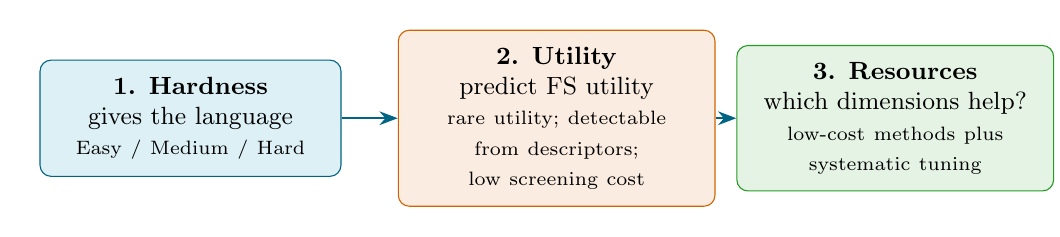
\begin{tikzpicture}[every node/.style={font=\small}]
  \useasboundingbox (-0.15,-1.15) rectangle (12.6,1.15);
  \node[box,text width=3.4cm,anchor=west] (a) at (0,0)
    {\textbf{1. Hardness}\\gives the language\\\scriptsize Easy / Medium / Hard};
  \node<2->[box,text width=3.6cm,anchor=west,fill=medorange!12,draw=medorange] (b) at (4.55,0)
    {\textbf{2. Utility}\\predict FS utility\\\scriptsize rare utility; detectable from descriptors; low screening cost};
  \node<3->[box,text width=3.6cm,anchor=west,fill=easygreen!12,draw=easygreen] (c) at (8.85,0)
    {\textbf{3. Resources}\\which dimensions help?\\\scriptsize low-cost methods plus systematic tuning};
  \draw<2->[arrow] (a) -- (b);
  \draw<3->[arrow] (b) -- (c);
\end{tikzpicture}

\onslide<4->{
\vspace{0.4cm}
\begin{center}
\small\color{bgucolor!80}
\textit{Dataset hardness provides a useful organizing variable for deciding
whether FS is useful and how resource-intensive the evaluation should be.}
\end{center}
}
\end{frame}

%% ── Open questions ───────────────────────────────────────────────────────────
\begin{frame}{Open research questions}

\begin{itemize}

\item Can we define a \textbf{generative model of datasets} that predicts
when iterative dataset peeling succeeds or fails in generating 'Hard' datasets?

\pause

\item What intrinsic properties explain the emergence of
'Hard' datasets, beyond simple dimensionality measures such as
the sample-to-feature ratio ($n/p$)?
    \pause


    \item Does feature-selection utility prediction generalize beyond tabular
    classification (e.g., time series, graphs)?

    \pause

    \item Explore how dataset complexity serves as a foundation for
    \textbf{resource-aware learning}, beyond feature selection?
\end{itemize}

\end{frame}

%% ── Thank you ────────────────────────────────────────────────────────────────
{
\setbeamertemplate{footline}{}
\begin{frame}
\vspace{0.7cm}
\begin{center}
{\Large\bfseries\color{bgucolor} Thank you}\\[6pt]
{\normalsize\color{gray} vilenchi@bgu.ac.il}\\[16pt]

\small
Published paper: \kbsfull\\[2pt]
\kbsdoi\ \,|\,\ \kbssd\\[10pt]
Code \& datasets: \repo\\[10pt]
\color{gray}Chapters~1--2 (utility prediction, resource-aware evaluation): under review.
\end{center}
\end{frame}
}



%% ── Backup: references ────────────────────────────────────────────────────────
\begin{frame}{References}
\footnotesize
\begin{itemize}\setlength{\itemsep}{3pt}
  \item M.\ J.\ Post, P.\ van der Putten, J.\ N.\ van Rijn.
        ``Does Feature Selection Improve Classification? A Large Scale Experiment
        in OpenML.'' \emph{Advances in Intelligent Data Analysis XV} (IDA 2016),
        LNCS 9897, 158--170. doi:10.1007/978-3-319-46349-0\_14.
  \item A.\ Bommert, X.\ Sun, B.\ Bischl, J.\ Rahnenf\"uhrer, M.\ Lang.
        ``Benchmark for filter methods for feature selection in high-dimensional
        classification data.'' \emph{Comput.\ Statist.\ Data Anal.}\ 143:106839,
        2020. doi:10.1016/j.csda.2019.106839.
  \item J.\ Li, K.\ Cheng, S.\ Wang, F.\ Morstatter, R.\ P.\ Trevino, J.\ Tang,
        H.\ Liu. ``Feature Selection: A Data Perspective.''
        \emph{ACM Comput.\ Surv.}\ 50(6):94, 2017. doi:10.1145/3136625.
  \item A.\ Filchenkov, A.\ Pendryak. ``Datasets meta-feature description for
        recommending feature selection algorithm.''
        \emph{AINL-ISMW FRUCT}, 11--18, 2015.
        doi:10.1109/AINL-ISMW-FRUCT.2015.7382962.
  \item A.\ R.\ S.\ Parmezan, H.\ D.\ Lee, F.\ C.\ Wu. ``Metalearning for choosing
        feature selection algorithms in data mining.''
        \emph{Expert Syst.\ Appl.}\ 75:1--24, 2017. doi:10.1016/j.eswa.2017.01.013.
  \item J.\ Komorniczak, P.\ Ksieniewicz. ``problexity --- An open-source Python
        library for supervised data complexity assessment.''
        \emph{Neurocomputing} 521:126--136, 2023. doi:10.1016/j.neucom.2022.11.056.
  \item I.\ Elmakias, D.\ Vilenchik. ``Choosing the Right Dataset: Hardness
        Criteria for Feature Selection Benchmarking.''
        \emph{Knowledge-Based Systems} 334:115022, 2026.
        doi:10.1016/j.knosys.2025.115022.
\end{itemize}
\end{frame}

\end{document}
